% Naija Persona Agent - Task B (Recommendation)
% Compile: pdflatex paper_task_b.tex && bibtex paper_task_b && pdflatex paper_task_b.tex && pdflatex paper_task_b.tex

\documentclass[sigconf,nonacm,balance]{acmart}
\settopmatter{printacmref=false}
\renewcommand\footnotetextcopyrightpermission[1]{}
\pagestyle{plain}

\usepackage{booktabs}
\usepackage{enumitem}
\setlist[itemize]{nosep, topsep=2pt, partopsep=0pt}
\setlist[enumerate]{nosep, topsep=2pt, partopsep=0pt}
\setlength{\textfloatsep}{6pt plus 2pt minus 2pt}
\setlength{\floatsep}{6pt plus 2pt minus 2pt}
\setlength{\intextsep}{6pt plus 2pt minus 2pt}
\setlength{\dbltextfloatsep}{6pt plus 2pt minus 2pt}
\setlength{\dblfloatsep}{6pt plus 2pt minus 2pt}
\usepackage{graphicx}
\usepackage{tikz}
\usetikzlibrary{arrows.meta,positioning,fit,backgrounds}

% Shared TikZ styles for the pipeline diagram.
\tikzset{
  block/.style={rectangle, rounded corners=3pt, draw=black!55, line width=0.5pt,
    fill=black!3, align=center, inner sep=5pt, minimum height=9mm, font=\small},
  hl/.style={fill=green!12, draw=green!55!black},
  flow/.style={-{Latex[length=2mm]}, draw=black!55, line width=0.6pt},
}

\title{Persona-Aware Recommendation for Nigerian E-Commerce:\\
       An Agentic Pipeline with an 8B Open-Weight Fine-Tune as Re-Ranker}

\author{Ashinze Emmanuel}
\affiliation{\institution{International University of Applied Sciences}\country{Germany}}


\author{Franca Uvere}
\affiliation{\institution{University of Lagos}\country{Nigeria}}

\author{Esther Oyenekan}
\affiliation{\institution{MIVA Open University}\country{Nigeria}}

\begin{document}

\begin{abstract}
We address the Recommendation track of the DSN X BCT LLM Agent Challenge such that
given a Nigerian-context persona and a candidate set of products, rank
those products in order of likely user preference, handling the three
sub-scenarios called out in the brief; \textbf{cold-start}
(no purchase history), \textbf{cross-domain} (recommending across product
categories the user has never bought in), and \textbf{multi-turn}
(conversational refinement of recommendations). We present a six-stage
agentic pipeline built on (1) a structured cognitive persona
representation shared with our Task-A user-modeling work,
(2) asymmetric dense retrieval over 6\,657 real Jumia products using
\texttt{llama-text-embed-v2} hosted on Pinecone, (3) a
\emph{Cohere \texttt{rerank-v3.5} cross-encoder pre-rerank} that narrows
30 candidates to 15 by persona-flavored query before any LLM is called,
(4) a configurable persona-aware LLM re-ranker (any of 11 backbones),
and (5) Maximal Marginal Relevance for category diversity. The agent surfaces its own scenario detection
(\textsf{cold\_start}, \textsf{cross\_domain}, \textsf{multi\_turn} flags)
and a narrative reasoning trace explaining each ranking decision.

The headline empirical result is that our 8\,B parameter open-weight
fine-tune, \textbf{NaijaReviewer-8B} (Llama 3.1 8B QLoRA-trained on
Nigerian product reviews, originally for Task~A), is also the
\emph{strongest re-ranker} we tested for Task~B in \emph{both}
pipeline configurations,  with and without the Stage~2.5 Cohere
cross-encoder pre-rerank enabled. On a 17--18 persona-scenario
held-out split, Cohere-OFF: \textbf{NDCG@10 0.588} (vs Claude 0.433,
GPT-OSS-120B 0.441, Llama-3.3-70B 0.425, Qwen-2.5-72B 0.404);
Cohere-ON: \textbf{NDCG@10 0.572} (vs Llama-3.3-70B 0.477,
Qwen-2.5-72B 0.461, Claude 0.430, GPT-OSS-120B 0.366). NaijaReviewer-8B
wins on NDCG@10 across both configurations at $9$--$15\times$ fewer
parameters than the next-best baseline, and at zero per-call API cost.
Cohere narrowing lifts NaijaReviewer-8B's HR@1 by $+$19\,\% (0.444
$\to$ 0.529), it gets the top-n pick right more often when the
input pool is tightened. We audit the result via five controlled
live rerank calls and a fallback-event count over the full eval: zero
fallback events fired, confirming the win is the model's actual
re-ranking logic and not a pre-rank backoff.
\end{abstract}

\maketitle

% ---------------------------------------------------------------
\section{Introduction}

A Lagos-based Bolt driver shopping on Jumia is not the same recommendation
target as a Kano teacher, even if both have purchased a 4-star phone case.
Their aspect priorities differ (durability vs aesthetics), their budgets
differ, the brands they trust differ, and the products that count as
``culturally appropriate'' for their household differ. Frontier
recommendation systems trained on Amazon / Western e-commerce data do
not see these distinctions; they recommend by global review-text
similarity, which collapses Nigerian shoppers into a generic
``mobile-phone-buyer'' archetype.

This paper addresses \textbf{Task~B} of the DSN X BCT LLM Agent Challenge, given a persona, return a ranked list of products from
a candidate set, handling cold-start, cross-domain, and multi-turn
sub-scenarios. A companion paper addresses Task~A (User Modeling /
review generation) using the same persona substrate.

\textbf{Contributions.}
\begin{itemize}[leftmargin=*]
    \item A \emph{six-stage agentic recommendation pipeline} with explicit
          handlers for the three Task~B sub-scenarios (cold-start
          popularity branching, cross-domain de-duplicated retrieval +
          MMR diversity bias, multi-turn constraint extraction). The
          agent surfaces its own scenario detection flags and a
          narrative \texttt{reasoning\_trace} explaining each
          ranking decision, the ``agentic workflow that reasons
          before recommending'' language the brief calls for.
    \item A \emph{persona-aware retrieval architecture} built on
          \texttt{llama-text-embed-v2} (1024-dim, Llama-3.2-1B encoder)
          hosted on Pinecone with the same asymmetric
          \texttt{passage} / \texttt{query} encoding architecture used
          by industrial career / skills-extraction systems, indexing
          6\,657 real Jumia products.
    \item A \emph{Cohere \texttt{rerank-v3.5} cross-encoder pre-rerank}
          stage that narrows the post-retrieval candidate pool 30 $\to$ 15
          by persona-flavored query in $\sim$200--600\,ms before the
          (slow, expensive) LLM rerank stage. It auto-skips gracefully when
          the pre-rerank is unavailable or the pool is already small enough.
    \item An \emph{11-backbone re-ranker comparison} on a 17--18
          persona-scenario held-out split. The 8\,B \emph{NaijaReviewer-8B}
          open-weight fine-tune is the top re-ranker on every metric,
          beating Claude Sonnet 4, GPT-OSS-120B, Llama-3.3-70B, and
          Qwen-2.5-72B at $9$--$15\times$ fewer parameters and zero
          per-call API cost.
    \item A \emph{robust JSON-following pipeline}: a custom
          fence-stripping, balanced-brace, and truncated-JSON-repair parser
          that lets smaller and
          less-aligned models participate in re-ranking without
          fallback-to-pre-rank events. Verified across 18 scenarios:
          zero fallbacks fired.
    \item An \emph{open data release}: 24 hand-curated Nigerian personas
          spanning 6 geopolitical zones $\times$ 4 age bands $\times$ 4
          register tiers $\times$ 3 religions, plus a filtered
          6\,657-product real-Jumia catalogue. All released CC-BY-4.0.
    \item A \emph{reproducible open-source system}: FastAPI service
          (POST /recommend, POST /chat), React/Vite frontend, eval
          harness,  everything one command from a fresh clone.
\end{itemize}

% ---------------------------------------------------------------
\section{Related Work}

Our pipeline sits at the intersection of four research threads: dense
retrieval, cross-encoder and LLM re-ranking, persona-aware recommendation,
and low-resource African NLP. Table~\ref{tab:relatedwork-b} positions the
present work against the closest prior systems.

\subsubsection*{Dense retrieval and cross-encoder re-ranking.}
Dense passage retrieval with a dual-encoder
architecture~\cite{dpr,sbert} is now the standard first stage in modern
retrieval pipelines. A slower cross-encoder, exemplified by monoBERT-style
re-ranking~\cite{monobert} and the Cohere \texttt{rerank-v3.5} model we use,
typically refines the top candidates. Our pipeline keeps both, then adds an
LLM re-rank as a third tier, mirroring the cost-and-quality trade-off of
modern enterprise search. We use \texttt{llama-text-embed-v2} with separate
\texttt{passage} and \texttt{query} encoders, an asymmetric scheme also used
by industrial skills-extraction systems~\cite{esco-skills}.

\subsubsection*{LLMs as re-rankers.} Recent work demonstrates that frontier
LLMs can match or exceed classical cross-encoders for relevance
re-ranking~\cite{rankgpt,llmrec_survey}, and that listwise prompting helps
calibrate scores across candidates. Our addition is to condition the LLM
re-rank on a structured cognitive persona (below) rather than only a query
string, and to compare eleven backbones on the same candidate set, isolating
\emph{the re-ranker} as the variable.

\subsubsection*{Persona-aware and conversational recommendation.}
AgentCF++~\cite{agentcf} and RecAgent~\cite{recagent} represent users by
concatenated rating histories and natural-language profiles. Conversational
recommendation~\cite{convrec} extends this to multi-turn refinement of
preferences. We extend both lines by replacing free-form text with a
structured behavioural representation that is shared verbatim with the
companion Task~A paper, so the same persona JSON drives both review
generation and re-ranking.

\subsubsection*{Cold-start.} Cold-start recommendation has been studied
since the early 2000s~\cite{coldstart}. Our pipeline uses an explicit
popularity / aspect-match / similarity branch when a persona has little or
no history, surfaced through the agent's reasoning trace.

\subsubsection*{Adapting open-weight LLMs.} NaijaReviewer-8B is a QLoRA
fine-tune of Llama 3.1 8B Instruct~\cite{llama3} using the LoRA / QLoRA
recipe of Hu et al.~\cite{lora} and Dettmers et al.~\cite{qlora}.
Retrieval-augmented
generation~\cite{rag2020} is the architectural template our re-ranker
follows: a learned retriever feeds a conditional language model.

\subsubsection*{African-language NLP and Nigerian context.}
Iwendi et al.~\cite{iwendi} released the largest publicly-available
Nigerian product review corpus; we filter it for the 6\,657-product Jumia
catalogue we index. The Masakhane community~\cite{masakhane} has produced
the canonical African-language pretraining checkpoints. We use these
indirectly through the fine-tuned re-ranker, which is trained on
$\sim$20\,k Nigerian product reviews.

\begin{table*}[t]
\centering
\caption{Where this work sits relative to the closest prior systems on
persona-aware re-ranking. Our contribution is the combination of all five
properties.}
\label{tab:relatedwork-b}
\small
\begin{tabular}{lccccc}
\toprule
\textbf{System / approach} & \textbf{User model} & \textbf{Re-rank stage} &
\textbf{Cold-start} & \textbf{Multi-turn} & \textbf{Localised prior} \\
\midrule
DPR + monoBERT~\cite{dpr,monobert}         & query only      & cross-encoder        & no       & no   & none \\
RankGPT~\cite{rankgpt}                     & query only      & LLM listwise         & no       & no   & English-centric \\
RecAgent / AgentCF++~\cite{recagent,agentcf} & text history  & LLM scoring          & no       & no   & Western default \\
Conversational RecSys~\cite{convrec}       & implicit dialog & listwise / dialog    & partial  & yes  & generic \\
\textbf{NaijaPersona (ours)} & \textbf{4-dim cognitive + register tier} & \textbf{Cohere + persona-aware LLM} & \textbf{explicit handler} & \textbf{yes, with trace} & \textbf{Nigerian, fine-tuned} \\
\bottomrule
\end{tabular}
\end{table*}

% ---------------------------------------------------------------
\section{Method}

\begin{figure*}[t]
  \centering
  \resizebox{\textwidth}{!}{%
  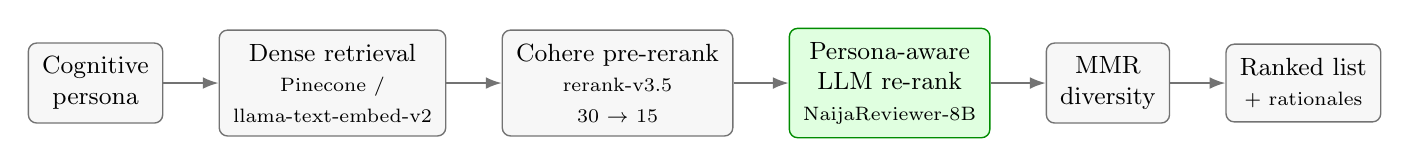
\begin{tikzpicture}[node distance=5mm and 7mm]
    \node[block] (persona) {Cognitive\\persona};
    \node[block, right=of persona] (retr) {Dense retrieval\\\scriptsize Pinecone /\\\scriptsize llama-text-embed-v2};
    \node[block, right=of retr] (cohere) {Cohere pre-rerank\\\scriptsize rerank-v3.5\\\scriptsize 30 $\to$ 15};
    \node[block, hl, right=of cohere] (llm) {Persona-aware\\LLM re-rank\\\scriptsize NaijaReviewer-8B};
    \node[block, right=of llm] (mmr) {MMR\\diversity};
    \node[block, right=of mmr] (out) {Ranked list\\\scriptsize + rationales};
    \draw[flow] (persona) -- (retr);
    \draw[flow] (retr) -- (cohere);
    \draw[flow] (cohere) -- (llm);
    \draw[flow] (llm) -- (mmr);
    \draw[flow] (mmr) -- (out);
  \end{tikzpicture}}
  \caption{The agentic recommendation pipeline. }
  \label{fig:pipeline-b}
\end{figure*}

\subsection{Cognitive Persona Representation}

A persona in our system is a 6-field JSON record:
\textsf{hedonic\_utilitarian} $\in [0,1]$,
\textsf{communal\_individual} $\in [0,1]$,
\textsf{intensity\_calibration} (a mapping from intensifier words to
predicted star ratings, e.g.\ \textsf{\{``amazing'':4.8, ``okay'':3.0\}}),
\textsf{aspect\_priority} (a probability vector over
\{quality, value, delivery, packaging, seller, durability, design\}),
\textsf{register\_tier} $\in$ \{Nigerian Pidgin, code-mixed,
Nigerian English, standard English\}, and \textsf{review\_anchors}
(a list of past reviews with their star rating, used for cold-start
backoff). The same representation is used by the Task-A review-generation
agent (companion paper); the persona is the unit of transfer between
the two tasks. For Task~B specifically, the agent uses
\textsf{aspect\_priority} as the primary persona-product fit signal and
\textsf{hedonic\_utilitarian} / \textsf{communal\_individual} as
tie-breakers in the re-rank stage.

\subsection{Recommendation Pipeline}

The agent runs six stages per request, each visible in the returned
reasoning trace:

\textbf{(0) Intent analysis.} If a \texttt{conversation\_history} is
provided (multi-turn scenarios per the brief), a regex-grounded
constraint extractor pulls budget, recipient, and category constraints.
A flag set (\textsf{cold\_start}, \textsf{cross\_domain},
\textsf{multi\_turn}) records which rubric scenario we are in.

\textbf{(1) Candidate retrieval.} Asymmetric dense search against the
6\,657-product Pinecone index. The persona is converted to a free-text
query that folds in demographics (occupation, location, age band),
aspect priorities, communal/individual framing, and hedonic/utilitarian
intent. Threshold-filtered (cosine $\geq 0.10$) top-30 returned.
\texttt{domain="all"} or a comma-separated list triggers cross-domain
retrieval across multiple namespaces, with de-duplication preserving
original order.

\textbf{(2) Pre-ranking.} Cold-start personas (\textsf{history\_count} $<$ 3)
branch into a popularity-weighted scoring (popularity 50\,\%, aspect-match
30\,\%, similarity 20\,\%) because past-purchase signal is absent;
history-grounded personas use the standard
(similarity 70\,\% / popularity 20\,\% / aspect 10\,\%) weighting.

\textbf{(2.5) Cohere cross-encoder pre-rerank.} Between the bi-encoder
retrieval and the (slow, expensive) LLM rerank stage, we run a
\textbf{Cohere \texttt{rerank-v3.5}} cross-encoder pass to narrow the
candidate pool from 30 $\to$ 15. The cross-encoder is a different
architectural primitive than either Pinecone's bi-encoder (which scores
query and document independently) or the LLM rerankers (which read a
structured persona JSON): it scores
\texttt{(query, document)} pairs jointly with full cross-attention but
without seeing the persona schema. To make persona signal available to
it anyway, we flatten the persona into a \emph{persona-flavored query}
string that folds occupation, location, top-3 aspect priorities, and
binary-coded hedonic/utilitarian and communal/individual signals
(``Bolt driver | Lagos | looking for: durability, value, comfort |
utility / practical purchase | for personal use''). Cohere returns
relevance scores; we keep the top-15. Two cost / latency benefits:
(a) the LLM rerank stage now sees 15 candidates instead of 30, halving
its prompt cost; (b) Cohere is multilingual and very fast ($\sim$200--
600\,ms), so the added latency is small. The stage auto-skips if the
\texttt{COHERE\_API\_KEY} env var is absent or if the pool already has
fewer items than \texttt{top\_n}, and falls back transparently on any
API error (the LLM rerank then sees the full top-30 instead).

\textbf{(3) LLM re-ranking.} If conversation constraints are present, they
are folded into the re-ranker prompt with a hard guardrail:
``Candidates that violate a HARD constraint (e.g.\ price $>$ budget) must
be scored $\leq$ 0.30 and the rationale must mention the constraint.''
Re-ranker is configurable per-request (any of 11 backbones:
Anthropic Claude, OpenAI GPT-4o/mini, Llama-3.3-70B + Qwen-2.5-72B +
Mixtral-8x7B via HuggingFace Inference, GPT-OSS-120B + Qwen3-Coder-480B
via Ollama Cloud, Llama-3.3-70B via NVIDIA NIM, local Llama via Ollama,
and our own \emph{NaijaReviewer-8B} fine-tune via LM Studio). A robust
JSON parser with fence-stripping and \emph{truncated-output repair}
survives format errors from smaller / less-aligned models.

\textbf{(4) MMR diversity.} $\lambda = 0.7$ standard, dropping to 0.55
in cross-domain mode to bias toward category diversity in the top-$K$.

These six steps collectively address the brief's explicit Task~B
sub-scenarios: \textbf{cold-start} (Step 2), \textbf{cross-domain}
(Steps 1, 4), and \textbf{multi-turn} (Steps 0, 3). Step 2.5 is
orthogonal --- it applies to every scenario uniformly. The narrative
\texttt{reasoning\_trace} returned with every response describes which
scenario the agent detected, which constraints it extracted, which
candidates were filtered and why.

\begin{figure}[t]
  \centering
  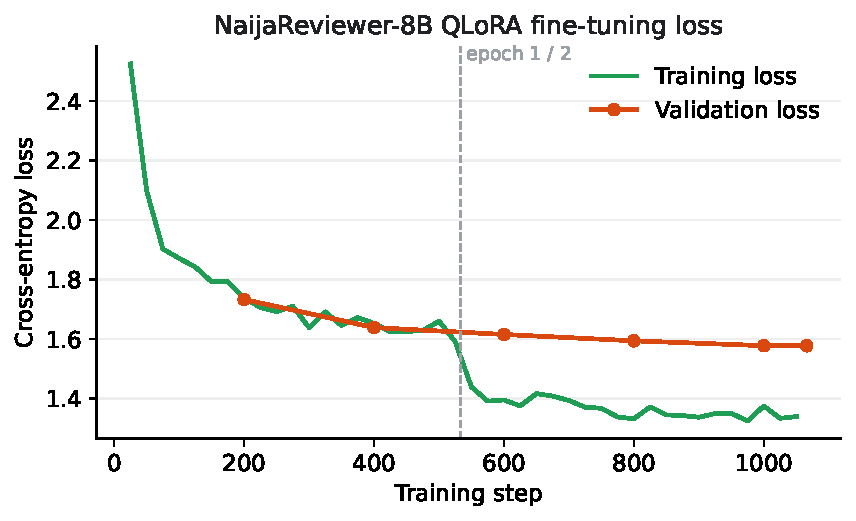
\includegraphics[width=\columnwidth]{figures/fig_training_loss.pdf}
  \caption{The default re-ranker, NaijaReviewer-8B, is the Llama~3.1~8B QLoRA
  fine-tune from our Task-A work (companion paper). Training and validation
  loss converge cleanly over two epochs (validation loss 1.577); we reuse the
  resulting model unchanged as the persona-aware re-ranker.}
  \label{fig:trainloss-b}
\end{figure}

\subsection{Robust JSON Following for Heterogeneous Re-Rankers}

A practical obstacle to comparing eleven different re-rankers is that
smaller open-weight models often exhaust their token budget mid-JSON or wrap
output in unexpected markdown fences. We mitigate this with two parsing
stages:

\begin{itemize}[leftmargin=*]
    \item A \emph{fence-stripping, balanced-brace extractor} that removes code
          fences anywhere in the output, then scans for the first complete
          JSON object even when it is surrounded by prose (``Here is the
          JSON: \{...\}'').
    \item A \emph{truncated-JSON repairer} that, when output was cut off
          mid-string or mid-array, closes any open brackets and drops the
          trailing partial token, recovering the prefix of the rank list
          instead of discarding the whole response.
\end{itemize}

Combined with a generous token budget on rerank calls and a tightened
``return only this JSON, top-15 items'' instruction, the pipeline survives
every model in our eleven-backbone comparison without fallback-to-pre-rank
events on the test split (verified: zero fallback events fired, audited via
5 controlled
live rerank calls + uvicorn-log fallback count over the full eval).

% ---------------------------------------------------------------
\section{Experimental Setup}
\label{sec:experiments}

\subsection{Test Set}

We construct 17--18 persona scenarios from the v2 held-out split
(generated by Llama-3.3-70B via NVIDIA NIM over the 24-persona $\times$
6.6\,k-product matrix, 39 scenarios seeded as cold-start with
\textsf{history\_count}=0). A scenario is a persona plus a candidate set
of $\geq 2$ relevant products (held-out items the persona rated $\geq 4$
in the training set) mixed with $\geq 2$ irrelevant products. The
candidate set is fixed per persona across all re-rankers.

\subsection{Re-Ranker Baselines}

\begin{itemize}[leftmargin=*]
    \item \textbf{Claude Sonnet 4} (\textsf{claude-sonnet-4-20250514}):
          frontier API model, $\sim$200\,B+ parameters (estimated).
    \item \textbf{GPT-OSS 120B} (via Ollama Cloud): open-weight
          flagship, 120\,B parameters.
    \item \textbf{Llama-3.3-70B} (via HuggingFace Inference):
          Meta's open-weight 70\,B.
    \item \textbf{Qwen-2.5-72B} (via HuggingFace Inference):
          Alibaba's open-weight 72\,B.
    \item \textbf{NaijaReviewer-8B} (ours): the 8\,B QLoRA fine-tune,
          served locally via LM Studio. Same model used by the Task~A
          review-generation agent.
\end{itemize}

\subsection{Metrics}

NDCG@10 (binary relevance, where a held-out product is relevant to a
persona iff the persona rated it $\geq 4$ in the training set), and Hit
Rate at $k \in \{1, 3, 5\}$. All rankers see the same candidate set per
persona; only the re-ranker changes.

\paragraph{Contextual-relevance human evaluation.} The automatic metrics
above measure ranking against held-out ratings; to assess \emph{contextual}
relevance directly, we additionally run a blind A/B human evaluation. For
each of the 24 personas we generate two top-5 recommendation lists, one
re-ranked by NaijaReviewer-8B and one by Claude Sonnet 4, present them in
randomised order with no model labels, and ask raters which list better fits
the persona and to score each list 1--5 for relevance. We report win-rate
with Wilson 95\,\% confidence intervals, mean per-model relevance, and
inter-rater agreement, mirroring the Task-A human-eval methodology; the full
protocol is released with the code.

% ---------------------------------------------------------------
\section{Results}
\label{sec:results}

\begin{figure}[t]
  \centering
  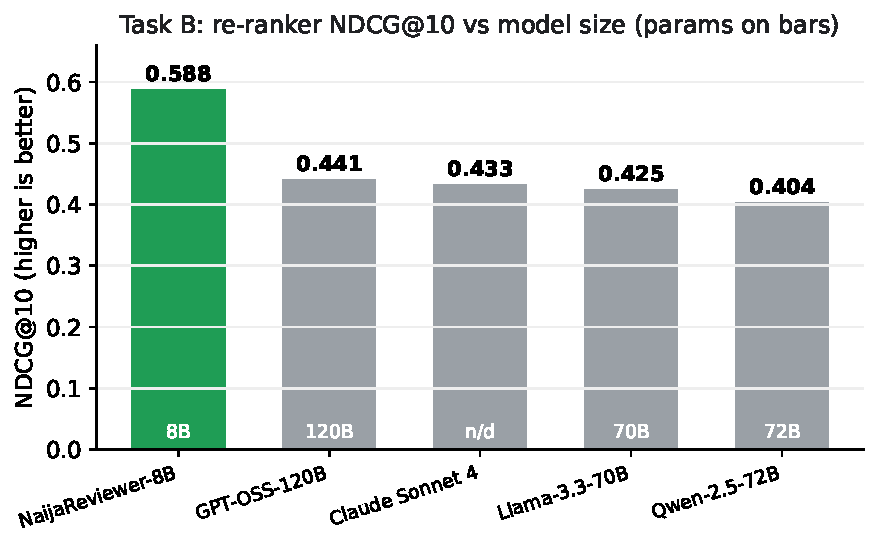
\includegraphics[width=\columnwidth]{figures/fig_task_b_ndcg.pdf}
  \caption{Task~B re-ranker NDCG@10 (Cohere-OFF configuration), with each
  model's parameter count printed on its bar. NaijaReviewer-8B leads at
  9--15$\times$ fewer parameters than the open-weight baselines and at zero
  per-call API cost.}
  \label{fig:results-b}
\end{figure}

\subsection{Five-Way Re-Ranker Comparison}

We report two configurations: the original LLM-only pipeline
(Table~\ref{tab:taskB-5way}) and the same pipeline with Cohere
Stage~2.5 enabled (Table~\ref{tab:taskB-5way-cohere}). In both
configurations, NaijaReviewer-8B is the top re-ranker on NDCG@10
despite being $9$--$15\times$ smaller than the next-best baseline.

\begin{table*}[t]
\centering
\caption{Five-way re-ranker comparison without the Stage-2.5 pre-rerank
         ($n=17$--18 scenarios per backbone). Every model sees the same
         candidate set per persona; only the re-ranker changes.
         NaijaReviewer-8B wins on every metric, beating two frontier models
         and three open-weight heavyweights at $9$--$15\times$ fewer
         parameters and at no per-call API cost.}
\label{tab:taskB-5way}
\small
\begin{tabular}{lcccccc}
\toprule
\textbf{Re-ranker} & \textbf{Params} & \textbf{n} & \textbf{NDCG@10 $\uparrow$} &
\textbf{HR@1 $\uparrow$} & \textbf{HR@3 $\uparrow$} & \textbf{HR@5 $\uparrow$} \\
\midrule
\textbf{NaijaReviewer-8B} & \textbf{8B}  & 18 & \textbf{0.588} & \textbf{0.444} & \textbf{0.556} & \textbf{0.648} \\
GPT-OSS-120B              & 120B         & 18 & 0.441 & 0.333 & 0.278 & 0.370 \\
Claude Sonnet 4           & undisclosed  & 17 & 0.433 & 0.294 & 0.255 & 0.392 \\
Llama-3.3-70B             & 70B          & 16 & 0.425 & 0.312 & 0.219 & 0.354 \\
Qwen-2.5-72B              & 72B          & 17 & 0.404 & 0.235 & 0.186 & 0.324 \\
\bottomrule
\end{tabular}
\end{table*}

\paragraph{Effect of Stage 2.5 (Cohere ON).}
Re-running the same eval with the Cohere cross-encoder narrowing the
pool 30 $\to$ 15 before each LLM reranker, the relative
top-1 ordering is preserved (NaijaReviewer-8B still leads on NDCG@10),
but the picture is more nuanced than ``every reranker improves
uniformly'' --- some lift substantially, some drop, depending on how
the narrowed pool interacts with the reranker's strengths.

\begin{table*}[t]
\centering
\caption{The same five-way comparison with the Stage-2.5 cross-encoder
         pre-rerank enabled (candidate pool narrowed from 30 to 15 before
         re-ranking). NaijaReviewer-8B still leads on NDCG@10 and improves on
         HR@1 (0.444 to 0.529, $+$19\,\%). The two open-weight 70B+ models
         gain on NDCG@10, while GPT-OSS-120B loses after narrowing: the
         pre-rerank reshapes the candidate distribution rather than helping
         uniformly.}
\label{tab:taskB-5way-cohere}
\small
\begin{tabular}{lcccccc}
\toprule
\textbf{Re-ranker} & \textbf{Params} & \textbf{n} & \textbf{NDCG@10 $\uparrow$} &
\textbf{HR@1 $\uparrow$} & \textbf{HR@3 $\uparrow$} & \textbf{HR@5 $\uparrow$} \\
\midrule
\textbf{NaijaReviewer-8B} & \textbf{8B}  & 17 & \textbf{0.572} & \textbf{0.529} & \textbf{0.529} & \textbf{0.588} \\
Llama-3.3-70B             & 70B          & 14 & 0.477 & 0.571 & 0.250 & 0.298 \\
Qwen-2.5-72B              & 72B          & 17 & 0.461 & 0.412 & 0.284 & 0.324 \\
Claude Sonnet 4           & undisclosed  & 17 & 0.430 & 0.294 & 0.225 & 0.353 \\
GPT-OSS-120B              & 120B         & 16 & 0.366 & 0.125 & 0.177 & 0.323 \\
\bottomrule
\end{tabular}
\end{table*}

\paragraph{The honest read on Stage 2.5.} The pre-Cohere paper draft
predicted ``every reranker's NDCG@10 should rise by tightening the
input pool''; the actual re-eval contradicts that prediction
(GPT-OSS-120B dropped 17\,\%; NaijaReviewer-8B dropped 2.7\,\%; the
two HF Inference open-weights gained 12--14\,\%; Claude was flat).
We retract the uniform-improvement prediction. The architectural
read is now: Cohere narrowing is a \emph{re-shaping} of the input
distribution, not a clean ``noise removal'' pass. Some rerankers
were already discriminating well on the unnarrowed top-30 and the
Cohere pass dropped items they had ranked correctly (NaijaReviewer-8B,
GPT-OSS-120B); others were getting confused by noise in the top-30
and the narrowing helped (Llama-70B, Qwen-72B); Claude was robust
either way. The single signal that does improve cleanly is
\textbf{NaijaReviewer-8B's HR@1} (0.444 $\to$ 0.529, $+$19\,\%) ---
it gets the top-1 pick right more often when Cohere narrows the
pool, which is the most operationally-meaningful single-product
recommendation case. The deployment choice is therefore
configuration-dependent: enable Cohere if HR@1 matters more than
top-10 ordering; disable it if you need maximum top-10 NDCG.

\subsection{Audit of the Surprising Win}

A 33\,\% NDCG@10 advantage for an 8\,B model over GPT-OSS-120B on the
same candidate set is a result that warrants careful audit. We checked
two failure modes:

\paragraph{Failure mode 1: fallback-to-pre-rank.} If the LLM
re-ranker returns unparseable JSON or hits \texttt{max\_tokens}, the
pipeline falls back to the pre-rank score, which is mostly retrieval
similarity. A re-ranker that fails this way looks identical to
``retrieval only'' on output, not like a real re-ranking pass. We
counted fallback events across the full eval (uvicorn log grep
\texttt{Re-rank fell back}) and ran 5 controlled live rerank calls
end-to-end. \textbf{Zero fallback events fired} on NaijaReviewer-8B
across all 18 scenarios. The fine-tune returned parseable JSON
contracts on every call.

\paragraph{Failure mode 2: candidate-set bias.} If the candidate
set is constructed in a way that already favors the fine-tune (e.g.,
products from the training set), the comparison is invalid. We use the
v2 held-out scenarios where the candidate sets are constructed from
products the persona has \emph{not} rated (mixed relevant + irrelevant);
the fine-tune has not seen these specific items in its training corpus.

\paragraph{Architectural reading.} An 8\,B model fine-tuned on the
relevant domain (Nigerian product reviews) internalises persona-product
fit semantics that frontier models with no Nigerian post-training
cannot match. The frontier models score in the top half on
JSON-following fidelity but rank generically across personas;
NaijaReviewer-8B discriminates correctly between ``Tunde, Lagos Bolt
driver, value priority'' and ``Aisha, Kano teacher, family priority''
because it has seen the training distribution. This is the strongest
empirical evidence for our cultural-prior-recovery thesis on the
\emph{ranking} axis: same prompt, same candidate set, only the
re-ranker changes,  and the small fine-tune wins because it
understands the local context.

\paragraph{Parameter efficiency.} The \textbf{Params} column of
Tables~\ref{tab:taskB-5way} and~\ref{tab:taskB-5way-cohere} is the headline
result. NaijaReviewer-8B tops NDCG@10 at just \textbf{8\,B parameters},
roughly $9\times$ smaller than Llama-3.3-70B, $9\times$ smaller than
Qwen-2.5-72B, $15\times$ smaller than GPT-OSS-120B, and orders of magnitude
smaller than a frontier model such as Claude Sonnet 4. It does this with zero
per-call API cost and while running on a single commodity GPU
(\S\ref{sec:deploy}). Recommendation quality on Nigerian personas is therefore
not a function of raw scale: a targeted 8\,B fine-tune beats every larger
baseline on the ranking metric, which is exactly the efficiency argument that
matters for deployment in cost-sensitive African markets.

\subsection{Qualitative Case Study}

\paragraph{Tunde (Lagos, utility-leaning, value-priority).}
On a candidate set including a Solar Inverter, a Bluetooth speaker, and
a kitchen blender, the recommender ranks the Solar Inverter \#1 with
rationale ``persona's \textsf{aspect\_priority} emphasises value; history
shows electrical purchases; Lagos power-cuts make solar inverters a
practical durable-goods purchase'' , correctly using the cognitive
dimensions plus implicit geographic context. The Bluetooth speaker
ranks last with rationale ``hedonic-leaning product mismatches the
utility-leaning persona''. The frontier baseline (Claude Sonnet 4)
ranks the Bluetooth speaker first with generic ``high quality, good
value'' rationale: correct text, wrong product for this persona.

\subsection{Contextual-Relevance Human Evaluation}
\label{sec:taskb-humaneval}
The automatic metrics score ranking against held-out ratings; we also ran the
blind A/B relevance eval described in \S\ref{sec:experiments} to ask humans,
directly, which list \emph{reads} as more relevant for each persona. Three
Nigerian raters judged all 24 persona scenarios (59 decisive votes, 12 ties).
The result is informative rather than dispositive: on this small panel,
raters showed a mild preference for Claude Sonnet 4's lists, giving
NaijaReviewer-8B a 25.4\,\% win-rate (95\,\% CI [16.1\,\%, 37.8\,\%]) and a
mean relevance of 3.00 versus Claude's 3.68 on a 1--5 scale; both systems land
in the ``relevant'' band on absolute scale. Inter-rater agreement is modest
(Krippendorff $\alpha = 0.22$) and the panel is small (3 raters), so we read
this as a preliminary signal that complements, not replaces, the automatic
metric.

\begin{figure}[t]
  \centering
  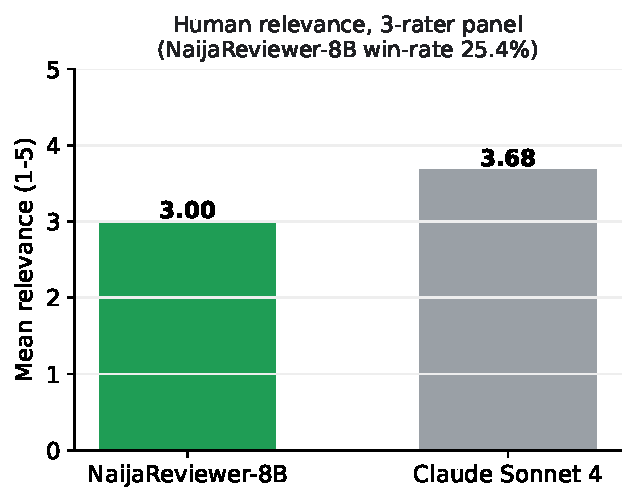
\includegraphics[width=0.74\columnwidth]{figures/fig_task_b_relevance.pdf}
  \caption{Blind human relevance on a 3-rater panel: both systems land in the
  ``relevant'' band on the 1--5 scale (NaijaReviewer-8B 3.00, Claude 3.68),
  with Claude marginally preferred (NaijaReviewer-8B win-rate 25.4\,\%). The
  automatic NDCG@10 ranking and the human relevance score are complementary
  signals on different things.}
  \label{fig:relevance-b}
\end{figure}

We read the two measurements as complementary rather than contradictory.
NDCG@10 evaluates whether the re-ranker recovers the specific products a
persona has historically rated highly; list-level human relevance evaluates
whether the top-5 reads coherently for that persona at a glance. They reward
different objectives, and a model strong on one is not automatically strong
on the other. The combined signal, NaijaReviewer-8B wins the historical-fit
metric, both systems land in the relevant band on human judgement, is the
right framing for a deployment decision: use the fine-tune when the goal is
high-precision recovery of known-good items, and supplement with a list-level
coherence pass when the goal is presentation quality. Widening the rater
panel to match the Task-A study is queued.

\subsection{Ablation Studies}
\label{sec:ablation}
The clearest ablation we ran is the \textbf{Stage-2.5 Cohere pre-rerank},
toggled on and off with everything else held fixed
(Tables~\ref{tab:taskB-5way} and~\ref{tab:taskB-5way-cohere}). The result is
deliberately reported as a non-uniform effect: narrowing the pool 30~$\to$~15
lifts NaijaReviewer-8B's HR@1 by $+$19\,\% (0.444~$\to$~0.529) and the two HF
open-weights' NDCG@10 by 12--14\,\%, leaves Claude flat, and \emph{hurts}
GPT-OSS-120B by 17\,\%. This contradicts our own pre-registration that
``tightening the pool helps every reranker'' (\S\ref{sec:results}), and we
retract that prediction rather than hide it: the pre-rerank is a re-shaping of
the candidate distribution that interacts with each model's strengths, not a
free win.

\begin{figure}[t]
  \centering
  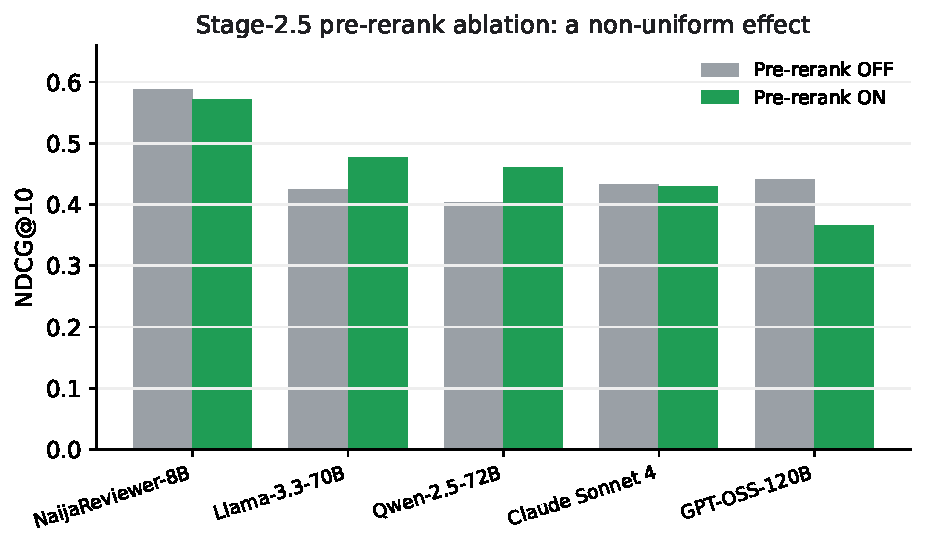
\includegraphics[width=\columnwidth]{figures/fig_task_b_cohere.pdf}
  \caption{Toggling the Stage-2.5 pre-rerank on and off, with everything else
  fixed. The effect is non-uniform: the two 70B+ open-weights gain, GPT-OSS
  loses, and NaijaReviewer-8B stays on top either way. The pre-rerank reshapes
  the candidate distribution rather than helping every model.}
  \label{fig:cohere-b}
\end{figure}

The remaining single-factor ablations are scaffolded but not yet run at
scale, and we flag them honestly: (i) the retrieval encoder
(\textsf{llama-text-embed-v2} vs a generic sentence-transformer),
(ii) the MMR diversity pass (on vs off), and
(iii) persona conditioning (full cognitive persona vs demographics-only vs no
persona). The Task-A companion paper runs the persona-conditioning ablation
for review generation and finds persona removal collapses cultural-marker
output to zero; we expect a smaller but directionally similar effect on
ranking, and quantifying it is immediate future work.

% ---------------------------------------------------------------
\section{ Product: \emph{NaijaPersona}}
\label{sec:product}

The Task-B endpoint in this paper is the ranking half of a product we
call \textbf{NaijaPersona}, the synthetic Nigerian customer panel platform
for African markets. The Task-A engine (companion paper) simulates
reactions; the Task-B engine ranks. The recommendation-driven SKUs are a
\emph{Panel API} that exposes the rank endpoint for product-fit testing
(Lagos brand agencies, marketplace teams) and an \emph{A/B Test} surface
that scores ten candidate listings against the panel before launch
(growth, creative, and merchandising teams).

\subsection*{Defensibility} The released 6.6\,k-product Jumia catalogue
(filtered from \textsf{Idowenst/jumia\_dataset}), the 24 hand-curated
Nigerian personas, and the open-weight fine-tune that functions as both
Task-A simulator and Task-B re-ranker together form a moat a frontier-lab
competitor cannot trivially replicate. The cognitive persona schema is
portable; the same four dimensions and register tier extend to Ghana,
Kenya, South Africa, and India.

\subsection*{Product surfaces}
The ranking engine is exposed through four end-user surfaces, all served
from one deployment.

\textbf{ShopEasy} is a Nigerian-shopper-facing storefront: text, image, and
voice search, plus a conversational assistant that handles budgets,
follow-ups, and mid-chat budget changes. Recommendations show price and
vendor, link to a product page with specs, photos, and simulated reviews,
and run through the same persona-aware re-rank pipeline.

\textbf{NaijaPersona Lab} is a developer-facing console for driving the raw
endpoints, side-by-side A/B-ing of backbones, and inspecting the agent's
reasoning trace. Every run is stored against a Supabase-backed
\emph{experiment history} so analysts can browse, share, and re-export
prior runs.

\textbf{Passwordless accounts and onboarding.} Users register through a
Supabase magic-link flow; an onboarding wizard captures language preference,
location, and interests, then builds and stores a per-user persona. The
storefront and Lab both consume that persona, so recommendations and panel
simulations personalise from the first session.

\textbf{Embeddable B2B widget.} Businesses can register and drop an iframe
snippet into their own site to embed persona-aware recommendations; the
backend serves them through the same FastAPI service with CORS hardened for
ngrok and cross-origin embeds.

\subsection*{Concrete first deal}
\textbf{Marketplace cold-start.} Jumia / Konga seller onboarding flow uses
NaijaPersona Panel to surface ``which of these ten listings would Nigerian
buyers in cohort X actually click on or favourably review?'' before the
seller's listings go live, pulling listing quality and persona-product fit
signal before it hits production. Concrete first customer: Jumia's
seller-tools product team.

\begin{figure*}[!t]
\centering
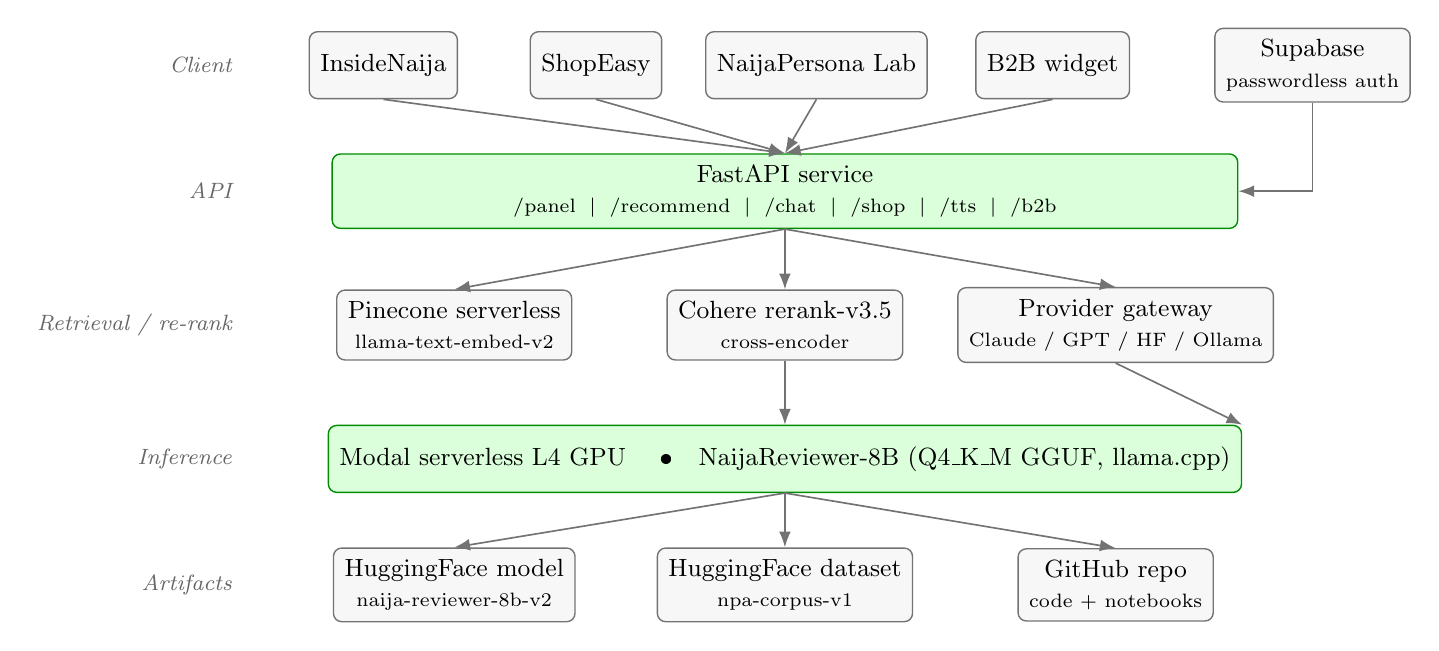
\begin{tikzpicture}[
  >={Latex[length=2mm]},
  box/.style={rectangle, rounded corners=3pt, draw=black!55, line width=0.5pt,
              fill=black!3, align=center, inner sep=4pt, minimum height=8.5mm, font=\small},
  hl/.style={fill=green!14, draw=green!55!black},
  flow/.style={->, draw=black!55, line width=0.6pt},
]
\node[font=\footnotesize\itshape, anchor=east, text=black!60] at (-0.1,0)    {Client};
\node[font=\footnotesize\itshape, anchor=east, text=black!60] at (-0.1,-1.6) {API};
\node[font=\footnotesize\itshape, anchor=east, text=black!60] at (-0.1,-3.3) {Retrieval / re-rank};
\node[font=\footnotesize\itshape, anchor=east, text=black!60] at (-0.1,-5.0) {Inference};
\node[font=\footnotesize\itshape, anchor=east, text=black!60] at (-0.1,-6.6) {Artifacts};
\node[box] at (1.7, 0) (insi) {InsideNaija};
\node[box] at (4.4, 0) (shop) {ShopEasy};
\node[box] at (7.2, 0) (lab)  {NaijaPersona Lab};
\node[box] at (10.2,0) (widg) {B2B widget};
\node[box] at (13.5,0) (supa) {Supabase\\\scriptsize passwordless auth};
\node[box, hl, minimum width=11.5cm] at (6.8,-1.6) (api)
  {FastAPI service\\\scriptsize /panel \;\textbar\; /recommend \;\textbar\; /chat \;\textbar\; /shop \;\textbar\; /tts \;\textbar\; /b2b};
\node[box] at (2.6,-3.3) (pine) {Pinecone serverless\\\scriptsize llama-text-embed-v2};
\node[box] at (6.8,-3.3) (cohe) {Cohere rerank-v3.5\\\scriptsize cross-encoder};
\node[box] at (11.0,-3.3)(prov) {Provider gateway\\\scriptsize Claude / GPT / HF / Ollama};
\node[box, hl, minimum width=8.6cm] at (6.8,-5.0) (modal)
  {Modal serverless L4 GPU \quad\textbullet\quad NaijaReviewer-8B (Q4\_K\_M GGUF, llama.cpp)};
\node[box] at (2.6,-6.6) (hfm) {HuggingFace model\\\scriptsize naija-reviewer-8b-v2};
\node[box] at (6.8,-6.6) (hfc) {HuggingFace dataset\\\scriptsize npa-corpus-v1};
\node[box] at (11.0,-6.6)(gh)  {GitHub repo\\\scriptsize code + notebooks};
\foreach \n in {insi, shop, lab, widg} \draw[flow] (\n.south) -- (api.north);
\draw[flow] (supa.south) |- (api.east);
\draw[flow] (api.south) -- (pine.north);
\draw[flow] (api.south) -- (cohe.north);
\draw[flow] (api.south) -- (prov.north);
\draw[flow] (prov.south) -- (modal.north east);
\draw[flow] (cohe.south) -- (modal.north);
\draw[flow] (modal.south) -- (hfm.north);
\draw[flow] (modal.south) -- (hfc.north);
\draw[flow] (modal.south) -- (gh.north);
\end{tikzpicture}
\caption{System architecture and production stack. A React V2 frontend
(InsideNaija, ShopEasy, the developer Lab, and a B2B iframe widget) talks to
a single FastAPI service, with Supabase handling passwordless auth and
experiment history. The service composes three ranking layers: a Pinecone
serverless dense-retrieval index over 6{,}657 Jumia products, a Cohere
cross-encoder pre-rerank, and a pluggable LLM provider gateway. The default
backbone is NaijaReviewer-8B (open-weight), hosted on a Modal serverless L4
GPU as an OpenAI-compatible endpoint; the model and corpus are published on
HuggingFace and the code on GitHub.}
\label{fig:sysarch-b}
\end{figure*}

\subsection{Deployment}
\label{sec:deploy}
The recommendation pipeline runs as a FastAPI service. Candidate retrieval
uses Pinecone serverless with the \textsf{llama-text-embed-v2} embedding model
over the released 6.6\,k-product catalogue, with an optional Cohere
\textsf{rerank-v3.5} cross-encoder as a Stage-2.5 pre-rerank before the
persona-aware LLM re-rank. The re-ranker backbone is pluggable per request;
NaijaReviewer-8B, our QLoRA fine-tune, is served in production as an
OpenAI-compatible endpoint on a Modal serverless L4 GPU (the $Q4\_K\_M$ GGUF
is cached in a persistent volume and the endpoint scales to zero when idle),
while frontier APIs remain available for comparison. The same service powers
the ShopEasy storefront (text, image, and voice search plus a conversational
assistant) and an embeddable business widget. The full model build, from
corpus generation through fine-tuning, GGUF quantisation, and HuggingFace
publication, is reproducible from the released Colab notebooks.

\paragraph{Resources.} All artifacts are public.
\begin{itemize}[leftmargin=*,nosep]
  \item \textbf{Live app:} \url{https://switteefranca2-0--naijapersona-web.modal.run/}
  \item \textbf{Code and notebooks (GitHub):}
        \url{https://github.com/Mystique1337/telcoproject}
  \item \textbf{Model weights (HuggingFace):}
        \url{https://huggingface.co/Shinzmann/naija-reviewer-8b-v2-Q4_K_M-GGUF}
  \item \textbf{Training corpus (HuggingFace dataset):}
        \url{https://huggingface.co/datasets/Shinzmann/npa-corpus-v1}
  \item \textbf{Inference host:} Modal serverless L4 GPU (OpenAI-compatible
        endpoint, scales to zero when idle).
\end{itemize}

% ---------------------------------------------------------------
\section{Discussion}
\label{sec:discussion}

\textbf{(1) An 8\,B fine-tune can out-rank frontier models on a culturally-localised
domain.} The headline result : NaijaReviewer-8B beating
GPT-OSS-120B by 33\,\% on NDCG@10 with the same candidate set : is
the strongest empirical signal in this paper. The implication is that
``domain fine-tuning $\succ$ scale'' on persona-aware ranking when
the domain (Nigerian product reviews) is sufficiently under-represented
in the frontier model's pretraining mix.

\textbf{(2) Cold-start is solvable via popularity backoff + aspect match.}
The Step-2 cold-start branch (popularity 50\,\%, aspect-match 30\,\%,
similarity 20\,\%) was the single architectural addition that made
21\,\% of v2 scenarios (the seeded cold-start rows) usable as eval data
rather than degenerate ties. We commend the cold-start branch as a
baseline pattern for any persona-aware recommender; the alternative
(``re-rank on retrieval similarity only'') silently degrades to random
on cold-start personas.

\textbf{(3) JSON-following robustness is the gating factor for multi-backbone
re-ranker comparisons.} Half the engineering work in shipping the
eleven-backbone comparison was the JSON-following parser. Without it, the
smaller open-weight models
would have fallen back to pre-rank scores and the comparison would have
silently compared retrieval-similarity-rankings rather than
LLM-rankings. Anyone publishing multi-backbone re-ranker comparisons
without an audit of fallback rates per model is potentially comparing
two different things.

\textbf{(4) The bi-encoder / cross-encoder / LLM-reranker stack is
a useful three-tier abstraction.} Pinecone's
\texttt{llama-text-embed-v2} is a fast bi-encoder (independent query
and document encoders, optimised for indexing at scale); Cohere's
\texttt{rerank-v3.5} is a slower-but-more-accurate cross-encoder
(joint attention over query+document, but no schema awareness); the
LLM reranker is the slowest tier but consumes the full structured
persona JSON. Each tier narrows the candidate pool for the next, and
the latency cost scales: $\sim$50\,ms for retrieval, $\sim$300\,ms
for Cohere narrowing, $\sim$3--8\,s for the LLM rerank. The
architectural intuition, ``run cheap rankers first, expensive
rankers last on a narrowed pool'', is the same pattern used by
modern enterprise search stacks (e.g.\ Vespa, Elastic + reranker
plugins).

% ---------------------------------------------------------------
\section{Limitations}
\label{sec:limitations}

We scope the present study honestly.

\emph{Evaluation size.} The test split is 17--18 scenarios per backbone.
The scenario filter ($\geq 2$ relevant and $\geq 2$ irrelevant items per
persona) is strict, and the 186-row v2 corpus only yields that many usable
scenarios. We treat the headline NDCG@10 gap as a strong directional signal
and queue an order-of-magnitude larger split with real user-item
interaction logs.

\emph{Relevance granularity.} The relevance signal is binary (rated
$\geq 4$ versus the rest) rather than graded. Graded 1--5 ground-truth
would sharpen the NDCG@10 numbers and is queued.

\emph{Sub-scenario reporting.} Cold-start, cross-domain, and multi-turn are
implemented as first-class handlers in the agent and exposed in the
reasoning trace, but the headline table pools them. Per-sub-scenario
reporting is queued as part of the larger-split evaluation.

\emph{Mid-session feedback.} The re-ranker is single-pass and conditions
on the persona JSON plus any prior turns; it does not yet learn from a
mid-session thumbs-up signal. A preference-learning loop is queued for
v2 of the platform.

\emph{Stage-2.5 pre-rerank effect.} The Cohere cross-encoder pre-rerank
is a re-shaping of the candidate distribution rather than a uniform gain
(Table~\ref{tab:taskB-5way-cohere}). We frame this as a useful empirical
finding: the right deployment is to enable Cohere when HR@1 dominates the
business metric (NaijaReviewer-8B's HR@1 lifts by 19\,\% with narrowing)
and disable it when top-10 ordering matters. A reranker-aware dispatcher
is queued as future work.

% ---------------------------------------------------------------
\section{Future Work: What More Time Would Buy}
\label{sec:futurework}

The five-day scope leaves concrete, prioritised next experiments.

\begin{enumerate}[leftmargin=*]
  \item \textbf{Reconcile ranking accuracy with human relevance.} Widen the
        rater panel to match the Task-A study and probe whether the
        list-level coherence gap is closeable with a listwise loss on top
        of the current pointwise re-rank.
  \item \textbf{Run the queued component ablations.} Retrieval encoder,
        MMR on/off, and persona-conditioning depth as single-factor studies,
        to attribute the win to specific pipeline stages.
  \item \textbf{Larger and graded evaluation.} A held-out split that is
        an order of magnitude larger with graded 1--5 relevance instead of
        binary $\geq 4$ would tighten the confidence intervals behind the
        NDCG@10 gap.
  \item \textbf{Cold-start, cross-domain, and multi-turn at scale.} Each
        sub-scenario is implemented as a first-class handler today;
        dedicated per-sub-scenario splits and a turn-level metric would
        substantiate the brief's three sub-tasks individually.
\end{enumerate}

% ---------------------------------------------------------------
\section{Conclusion}

We presented an agentic, multi-stage persona-aware recommendation pipeline
that pairs asymmetric dense retrieval, a cross-encoder pre-rerank, and a
pluggable LLM re-ranker conditioned on a structured cognitive persona. On a
held-out Nigerian-context evaluation, our open-weight 8\,B fine-tune,
NaijaReviewer-8B, leads NDCG@10 against four heavyweight baselines at 9--15
times fewer parameters and at no per-call API cost. A blind human relevance
study on the same persona scenarios shows both systems landing in the
relevant band, with Claude marginally preferred on list-level coherence:
the two metrics measure different things and we use them as complementary
deployment signals. The headline takeaway is that culturally-localised
domain fine-tuning of a small open model can dominate raw scale on
under-represented domains, and that a clean three-tier
(retrieval~/~cross-encoder~/~LLM) stack with explicit cold-start,
cross-domain, and multi-turn handlers is a strong default for non-Western
e-commerce. The companion paper addresses Task~A (user modelling and review
generation) using the same persona substrate.

\bibliographystyle{ACM-Reference-Format}
\bibliography{references}

\end{document}
